\documentclass[crop,tikz]{standalone}
\usetikzlibrary{arrows.meta}
\tikzstyle{myarrows}=[line width=1mm,draw=blue,-triangle 45,postaction={draw, line width=3mm, shorten >=4mm, -}]
\begin{document}

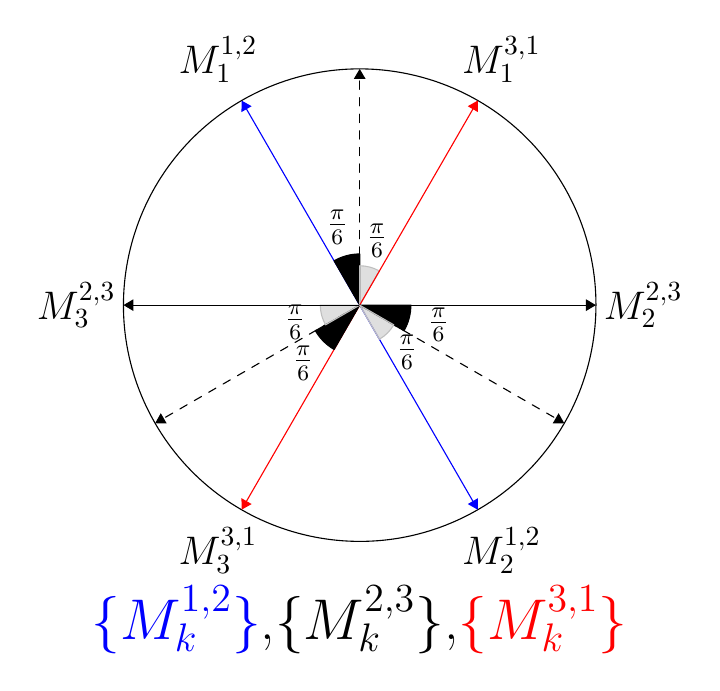
\begin{tikzpicture}[line cap=round, line join=round, >=Triangle]




\begin{scope}[ shift={(5,-7)},rotate=30]
\draw  (0,0) ellipse (3 and 3);


\draw[->,color=blue]  (0,0) -- (0,3);
\draw[->,dashed,rotate=-30]  (0,0) -- (0,3);
\draw[->,color=blue]  (0,0) -- (0,-3);
\draw (0,3.6) node {\Large $M^{1,2}_1$};
\draw (0,-3.6) node {\Large $M^{1,2}_2$};
\draw [shift={(0,0)}, fill] (0,0) -- (90:0.65) arc (90:60:0.65) -- cycle;
\node at (0.6,0.6) {\large $\frac{\pi}{6}$};
\draw [shift={(0,0)}, lightgray, fill, fill opacity=0.5] (0,0) -- (60:0.5) arc (60:30:0.5) -- cycle;
\node at (0.25,1) {\large $\frac{\pi}{6}$};


\begin{scope}[rotate=120]
\draw[->,dashed,rotate=-30]  (0,0) -- (0,3);
    \draw[->,color=red]  (0,0) -- (0,3);
    \draw[->,color=red]  (0,0) -- (0,-3);
	\draw (0,3.6) node {\Large $M^{3,1}_3$};
	\draw (0,-3.6) node {\Large  $M^{3,1}_1$};
	\draw [shift={(0,0)}, fill] (0,0) -- (90:0.65) arc (90:60:0.65) -- cycle;
\node at (0.6,0.6) {\large $\frac{\pi}{6}$};
\draw [shift={(0,0)}, lightgray, fill, fill opacity=0.5] (0,0) -- (60:0.5) arc (60:30:0.5) -- cycle;
\node at (0.25,1) {\large $\frac{\pi}{6}$};

\end{scope}

\begin{scope}[rotate=240]    
\draw[->,dashed,rotate=-30]  (0,0) -- (0,3);
	 \draw[->,color=black]  (0,0) -- (0,3);
    \draw[->,color=black]  (0,0) -- (0,-3);
	\draw (0,3.6) node {\Large $M^{2,3}_2$};
	\draw (0,-3.6) node {\Large $M^{2,3}_3$};
	\draw [shift={(0,0)}, fill] (0,0) -- (90:0.65) arc (90:60:0.65) -- cycle;
\node at (0.6,0.6) {\large $\frac{\pi}{6}$};
\draw [shift={(0,0)}, lightgray, fill, fill opacity=0.5] (0,0) -- (60:0.5) arc (60:30:0.5) -- cycle;
\node at (0.25,1) {\large $\frac{\pi}{6}$};
;
\end{scope}

\end{scope}

\node at (5,-11) {\huge {\color{blue} $\{M^{1,2}_k\}$},{\color{black} $\{M^{2,3}_k\}$},{\color{red} $\{M^{3,1}_k\}$}};

\end{tikzpicture}

\end{document}